\documentclass[12pt,a4paper,bibliography=totocnumbered,listof=totocnumbered]{scrartcl}
\usepackage[ngerman]{babel}
\usepackage[utf8]{inputenc}
\usepackage{amsmath}
\usepackage{amsfonts}
\usepackage{amssymb}
\usepackage{graphicx}
\usepackage{fancyhdr}
\usepackage{tabularx}
\usepackage{geometry}
\usepackage{setspace}
\usepackage[right]{eurosym}
\usepackage[printonlyused]{acronym}
\usepackage{subfig}
\usepackage{floatflt}
\usepackage[usenames,dvipsnames]{color}
\usepackage{colortbl}
\usepackage{paralist}
\usepackage{array}
\usepackage{titlesec}
\usepackage{parskip}
\usepackage[right]{eurosym}
\usepackage{picins}
\usepackage[subfigure,titles]{tocloft}
\usepackage[pdfpagelabels=true]{hyperref}

\usepackage{listings}
\inputencoding{utf8}
\lstset{basicstyle=\footnotesize, captionpos=b, breaklines=true, showstringspaces=false, tabsize=2, frame=lines, numbers=left, numberstyle=\tiny, xleftmargin=2em, framexleftmargin=2em}
\makeatletter
\def\l@lstlisting#1#2{\@dottedtocline{1}{0em}{1em}{\hspace{1,5em} Lst. #1}{#2}}
\makeatother

\geometry{a4paper, top=27mm, left=30mm, right=20mm, bottom=35mm, headsep=10mm, footskip=12mm}

\hypersetup{unicode=false, pdftoolbar=true, pdfmenubar=true, pdffitwindow=false, pdfstartview={FitH},
	pdftitle={Lobbyarbeit im digitalen Zeitalter},
	pdfauthor={Marco Seidler},
	pdfsubject={Lobbyarbeit},
	pdfcreator={\LaTeX\ with package \flqq hyperref\frqq},
	pdfproducer={pdfTeX \the\pdftexversion.\pdftexrevision},
	pdfkeywords={Lobbyarbeit},
	pdfnewwindow=true,
	colorlinks=true,linkcolor=black,citecolor=black,filecolor=magenta,urlcolor=black}
\pdfinfo{/CreationDate (D:20110620133321)}

\begin{document}

\titlespacing{\section}{0pt}{12pt plus 4pt minus 2pt}{-6pt plus 2pt minus 2pt}

% Kopf- und Fusszeile
\renewcommand{\sectionmark}[1]{\markright{#1}}
\renewcommand{\leftmark}{\rightmark}
\pagestyle{fancy}
\lhead{}
\chead{}
\rhead{\thesection\space\contentsname}
\lfoot{Lobbyarbeit im digitalen Zeitalter}
\cfoot{}
\rfoot{\ \linebreak Seite \thepage}
\renewcommand{\headrulewidth}{0.4pt}
\renewcommand{\footrulewidth}{0.4pt}

% Vorspann
\renewcommand{\thesection}{\Roman{section}}
\renewcommand{\theHsection}{\Roman{section}}
\pagenumbering{Roman}

% ----------------------------------------------------------------------------------------------------------
% Titelseite
% ----------------------------------------------------------------------------------------------------------
\thispagestyle{empty}
\begin{center}
	
\includegraphics[scale=1]{Bilder/hs_os.jpg}\\
	\vspace*{2cm}
	\Large
	\textbf{Hochschule für Wirtschaft und Technik, Berlin}\\
	\vspace*{2cm}
	\Huge
	\textbf{Semesterarbeit}\\
	\vspace*{0.5cm}
	\large
	über das Thema\\
	\vspace*{1cm}
	\textbf{Lobbyarbeit im digitalen Zeitalter: was wird, was muss sich verändern?}\\
	\vspace*{2cm}
	
	\vfill
	\normalsize
	\newcolumntype{x}[1]{>{\raggedleft\arraybackslash\hspace{0pt}}p{#1}}
	\begin{tabular}{x{6cm}p{7.5cm}}
		\rule{0mm}{5ex}\textbf{Autor:} & Marco Seidler \\ 
		\rule{0mm}{5ex}\textbf{Matrikelnummer:} & 547431 \\ 
		%\rule{0mm}{5ex}\textbf{Betreuerin:} & Prof. Dr. Debora Weber-Wulff \\ 
		\rule{0mm}{5ex}\textbf{Abgabedatum:} & 28.10.2015 \\ 
	\end{tabular} 
\end{center}
\pagebreak

% ----------------------------------------------------------------------------------------------------------
% Abstract
% ----------------------------------------------------------------------------------------------------------
\setcounter{page}{1}
\onehalfspacing
\titlespacing{\section}{0pt}{12pt plus 4pt minus 2pt}{2pt plus 2pt minus 2pt}
\rhead{KURZFASSUNG}
\section{Kurzfassung}
Im Rahmen dieser Arbeit wurde auf die Thematiken Lobbyismus und digitales Zeitalter eingegangen. Es wurden jeweils die wichtigsten Begriffe geklärt und auf die Thematik der Digitalisierung der Gesellschaft mit Bezug auf den Lobbyismus eingegangen. Dafür wurden auch Beispiele der Praxis betrachtet und diese in Bezug zur aktuellen Entwicklung gesetzt. Zuletzt erfolgte ein Fazit über die gewonnenen Erkenntnisse.  

\pagebreak

% ----------------------------------------------------------------------------------------------------------
% Verzeichnisse
% ----------------------------------------------------------------------------------------------------------
% TODO Typ vor Nummer
\renewcommand{\cfttabpresnum}{Tab. }
\renewcommand{\cftfigpresnum}{Abb. }
\settowidth{\cfttabnumwidth}{Abb. 10\quad}
\settowidth{\cftfignumwidth}{Abb. 10\quad}

\titlespacing{\section}{0pt}{12pt plus 4pt minus 2pt}{2pt plus 2pt minus 2pt}
\singlespacing
\rhead{INHALTSVERZEICHNIS}
\renewcommand{\contentsname}{II Inhaltsverzeichnis}
\phantomsection
\addcontentsline{toc}{section}{\texorpdfstring{II \hspace{0.35em}Inhaltsverzeichnis}{Inhaltsverzeichnis}}
\addtocounter{section}{1}
\tableofcontents
\pagebreak
\rhead{VERZEICHNISSE}
\listoffigures
\pagebreak

%\pagebreak
%\renewcommand{\lstlistlistingname}{Listing-Verzeichnis}
%{\labelsep2cm\lstlistoflistings}
%\pagebreak

% ----------------------------------------------------------------------------------------------------------
% Inhalt
% ----------------------------------------------------------------------------------------------------------
% Abstände Überschrift
\titlespacing{\section}{0pt}{12pt plus 4pt minus 2pt}{-6pt plus 2pt minus 2pt}
\titlespacing{\subsection}{0pt}{12pt plus 4pt minus 2pt}{-6pt plus 2pt minus 2pt}
\titlespacing{\subsubsection}{0pt}{12pt plus 4pt minus 2pt}{-6pt plus 2pt minus 2pt}

% Kopfzeile
\renewcommand{\sectionmark}[1]{\markright{#1}}
\renewcommand{\subsectionmark}[1]{}
\renewcommand{\subsubsectionmark}[1]{}
\lhead{Kapitel \thesection}
\rhead{\rightmark}

\onehalfspacing
\renewcommand{\thesection}{\arabic{section}}
\renewcommand{\theHsection}{\arabic{section}}
\setcounter{section}{0}
\pagenumbering{arabic}
\setcounter{page}{1}

% ----------------------------------------------------------------------------------------------------------
% Einleitung
% ----------------------------------------------------------------------------------------------------------
\section{Einleitung}
Diese vorliegende Arbeit umfasst als Thematiken den Lobbyismus sowie die Relevanz und die Auswirkungen der Entwicklung und Verbreitung des Web 2.0 auf die Branche. 
Es stellt sich dabei die Frage wie Lobbyismus zu früheren Zeiten abgehalten wurde und wie die Digitalisierung der Gesellschaft sich auf dieses traditionelle Vorgehen auswirkt. 
Können die Verbände der Lobbyisten dieser schnellen Entwicklung standhalten?  
In den folgenden Seiten soll daher dargelegt werden, wie das Vorgehen bei dem Ausüben des Lobbyismus traditionell erfolgt und wie die Digitalisierung sich auf dieses ausübt. 

\pagebreak

% ----------------------------------------------------------------------------------------------------------
% Kapitel
% ----------------------------------------------------------------------------------------------------------
\section{Begriffsklärung}

Nachfolgend wird auf wichtige Begriffe zur Abgrenzung der Bedeutung von Teilaspekten dieser Arbeit eingegangen.
Die erste Frage die sich im Rahmen dieser Arbeit stellt ist: „Was ist Lobbyismus?“. 
Nach Carsten Bockstette ist Lobbyismus folgendermaßen definiert: „Lobbyismus ist der Versuch der Einflussnahme auf Entscheidungsträger durch Dritte.“ \cite[vgl. S.18]{KNEV03}. Etwas genauer definiert es Alexander Bilgeri, er beschreibt das Lobbying als „eine direkte bzw. indirekte Einflussnahme auf politische Prozesse von Organisationen durch externe Teilnehmer – auch mit Hilfe von Machtgrundlagen – zur Verfolgung eines bestimmten Zwecks“ \cite[S.13]{DPL01}.  Dies ist eine recht treffende Beschreibung und zeigt vor allem die Zweckorientierung der Lobbyarbeit auf.
Im Zuge dieser Arbeit wird analysiert werden, wie diese Einflussnahme vonstattengeht.
In den Medien ist immer häufiger von dem „digitalen Zeitalter“ – auch mit dem sogenannten Web 2.0 - die Rede. Es stellt sich die Frage was verbirgt sich hinter diesen abstrakten Begriffen?
Es wird vermutet, dass es das erste Mal im Jahr 2002 möglich war, mehr Informationen digital als im Analogformat zu speichern \cite[vgl .S.60–65]{WTC11} , weshalb dies als der Beginn des „Digitalen Zeitalters“ angesehen werden kann.  Der Begriff Web 2.0 bezieht sich neben spezifischen Technologien oder Innovationen wie Cloud-Computing primär auf eine veränderte Nutzung und Wahrnehmung des Internets. \cite[vgl.]{EIWP} 
Hierbei sind die Nutzer selber aktiv und erstellen, verteilen digitale Inhalte interaktiv. Ein wichtiger Trend dessen sind die Sozialen Medien – Twitter, Facebook und co. – welche im Rahmen dieser Arbeit einen hohen Stellenwert einnehmen. 

\pagebreak

% ----------------------------------------------------------------------------------------------------------
% Kapitel
% ----------------------------------------------------------------------------------------------------------
\section{Öffentlichkeitsarbeit in der Praxis}

Wie wird von den Lobbyisten nun die Öffentlichkeitsarbeit im Web 2.0 genutzt? 
Es soll daher geklärt werden wie die allgemeine Verwendung der Digitalen Infrastruktur dem Lobbyismus nützen kann und inwiefern dies schon in den Verbänden vertreten ist.
Der Stellenwert der Öffentlichkeitsarbeit hat in den letzten Jahren deutlich zugenommen, so ist es Verbänden möglich, über gezielte Mediennutzung eine große Anzahl potentieller Nutzer anzusprechen. 
Bei einer Veranstaltung des Arbeitskreises Verbandskommunikationen im November 2014 wurde unter Vertretern verschiedener Verbände das Thema „Digital Lobbying“ behandelt. 
Matthias Banner von dem Bunderverband der Dienstleistungswirtschaft e.V (BDWi) zeigt dabei auf, wie der BDWI seine Interessen durchsetzt. Er schaffe Reichweite für die Themen der Mitgliedsverbände, indem er Content produziere und Events organisiere, sowie deren Verbreitung befördere. Dabei wird speziell auf das entsprechende Nutzungsverhalten eines Stakeholders eingegangen. Das kann über die Webseite, Newsletter, Facebook und Twitter erfolgen. \cite[vgl.]{DPRG}

\vspace{1em}
\begin{minipage}{\linewidth}
	\centering
	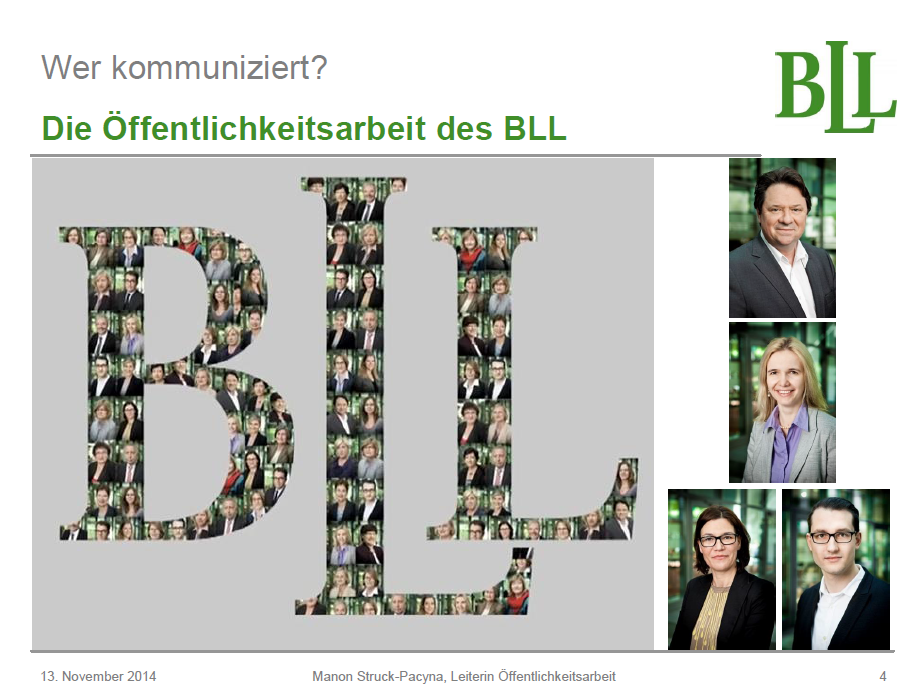
\includegraphics[width=1\linewidth]{Bilder/bla1.png}
	\captionof{figure}[Die Öffentlichkeitsarbeit des BLL]{Die Öffentlichkeitsarbeit des BLL\footnotemark }
	\label{fig:osgi}
\end{minipage}
\footnotetext{Quelle: \cite{DPRGB}}

Eine weitere Vertreterin war Manon Struck-Pacyna von dem Bund für Lebensmittelrecht und Lebensmittelkunde e.V. (BLL).

Diese kristallisiert das Vorgehen des BLL in Sachen Digital Lobbying der BLL heraus. Lange Zeit fand diese ausschließlich auf klassische Weise in Form von Veranstaltungen, Hintergrundgesprächen, Newslettern etc. statt. Doch seit Anfang 2014 bringt der BLL seine hohe fachliche Expertise auch digital ein“, schilderte Struck-Pacyna die Ausgangslage. Dabei seien die Verbands-Webseite mit Adaptierung für die Mobile Darstellung im Responsive Design sowie guter SEO (search engine  optimization) und der Twitter-Kanal @BLL\_de ein wichtiger Bestandteil des Daily Business geworden und aufgrund dessen auch nicht mehr wegzudenken. „Gerade auf Twitter sind viele wichtige Politiker und politische Organisationen aktiv. Egal ob als Live-Kommunikation von Veranstaltungen mit politischen Gästen oder themenspezifische Interaktion über direkte Ansprache oder klug gewählte Hashtags – schneller und vor allem für die Öffentlichkeit transparenter als über Twitter kann man Abgeordnete heutzutage nicht erreichen“ schilderte Frau Pacyna. \cite[vgl.]{DPRG}

\vspace{1em}
\begin{minipage}{\linewidth}
	\centering
	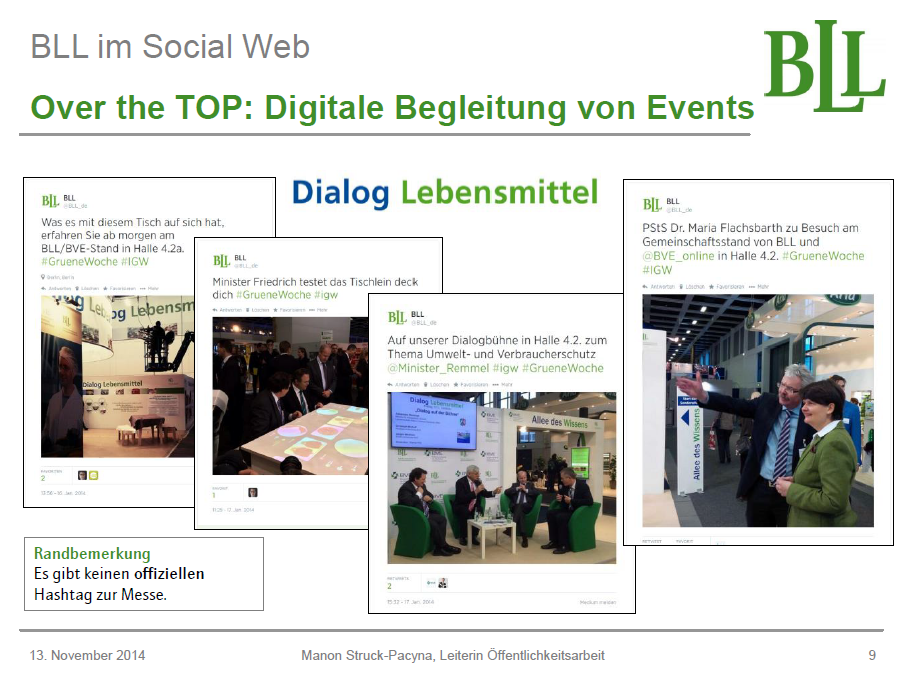
\includegraphics[width=1\linewidth]{Bilder/bla2.png}
	\captionof{figure}[BLL digitale Begleitung von Events]{BLL digitale Begleitung von Events\footnotemark }
	\label{fig:osgi}
\end{minipage}
\footnotetext{Quelle: \cite{DPRGB}}

Zusammenfassend kommunizierte Christian H. Schuster von der IFK Berlin „Facebook und Twitter können die klassischen Lobbying-Instrumente nicht ersetzen. Für einen modernen Verband sind die sozialen Netzwerke eine sinnvolle Ergänzung. Verbände können sowohl Politikern und Mitgliedern, als auch der Öffentlichkeit zeigen, dass sie die politische Interessenvertretung ernst nehmen und auch im digitalen Raum als Sprachrohr der Mitglieder fungieren“. \cite[vgl.]{DPRG}

\pagebreak

% ----------------------------------------------------------------------------------------------------------
% Kapitel
% ----------------------------------------------------------------------------------------------------------
\section{Reflektion zur Öffentlichkeitsarbeit}

Die Ursprungsfrage lautete: „Lobbyarbeit im digitalen Zeitalter: was wird, was muss sich verändern?“. Es ist gesichert, dass wir seit dem Jahr 2002 das digitale Zeitalter schreiben. Die Gesellschaft befindet sich im Wandel, die Digitalisierung nimmt immer weiter zu und ebenso müssen sich die Unternehmen und auch die Verbände mitentwickeln. Dem Trend entgegenzusteuern ist keine Option mehr, weshalb die Verbände nun ebenfalls vermehrt auf die Digitalisierung setzen müssen. Dabei spielen viele Faktoren eine Rolle, die verwendeten Kanäle, das Mithalten in aktuellen Disziplinen der Technik – siehe SEO – und das Aufbauen einer Webpräsenz. Klassischer Lobbyismus wird durch diesen Trend höchstwahrscheinlich nicht abgelöst werden, aber er wird sich immer weiter      an die digitale Gesellschaft anpassen müssen um bestehen zu bleiben. 
Viele Verbände haben bereits weitreichende Veränderungen gestartet um dem aktuellen Trend gerecht zu werden. Der Bund für Lebensmittelrecht und Lebensmittelkunde e.V. (BLL) ist hier ein gutes Beispiel wie eine digitale Agenda vorangetrieben werden kann und eine Webpräsenz – auch in social Media – geschaffen und erhalten werden kann. Der Nutzen dessen ist unverkennbar, neben dem Aufbau größerer Netzwerke wird auch eine große Basis der potenziellen Nutzer der Produkte des Verbandes angesprochen.


Es gibt inzwischen eigene Agenturen, welche als Geschäftsmodell ausschließlich das Näherbringen des Digital Lobbying an Verbände haben. Ein Beispiel hierfür ist die IFK (\url{http://agentur-adverb.de/}), welche eigens Magazine mit diesen Thematiken publizieren. Auch dies zeigt eindeutig auf, dass sich der Trend stark zur Digitalisierung hinbewegt. 

\vspace{1em}
\begin{minipage}{\linewidth}
	\centering
	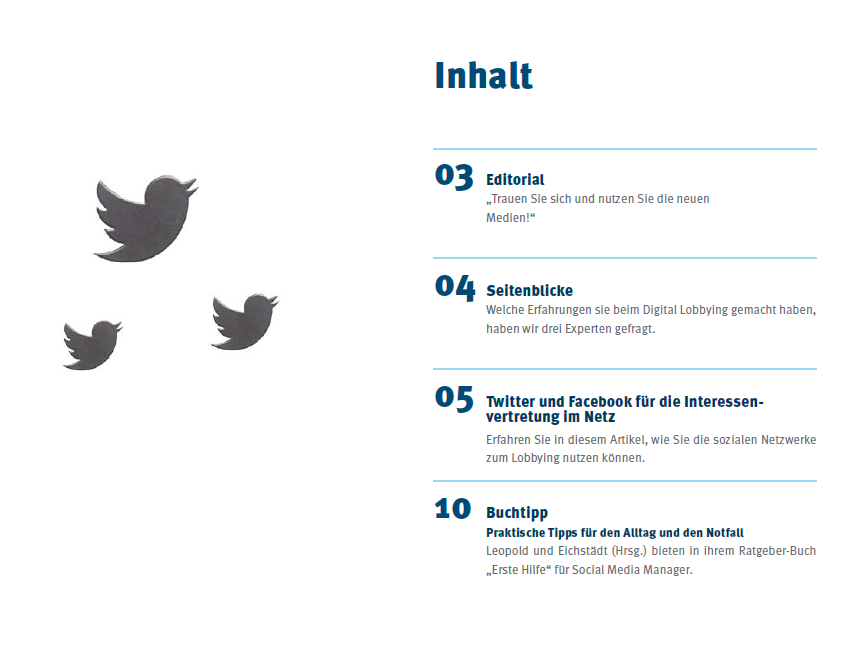
\includegraphics[width=1\linewidth]{Bilder/bla3.png}
	\captionof{figure}[Inhalt des "`Digital Lobbying"' Magazin der IFK ]{Inhalt-des "`Digital Lobbying"' Magazin der IFK\footnotemark }
	\label{fig:osgi}
\end{minipage}
\footnotetext{Quelle: \cite{AAD}}

\pagebreak

% ----------------------------------------------------------------------------------------------------------
% Kapitel
% ----------------------------------------------------------------------------------------------------------
\section{Fazit}

Die Digitalisierung der Gesellschaft nimmt stetig zu und Verbände müssen ihre Strategien überdenken um mit diesem Trend mithalten zu können. Die klassischen Methoden sind durchaus noch vertreten, aber sollten im Web 2.0 nicht mehr alleiniges Merkmal eines Verbandes sein. 

\pagebreak

% ----------------------------------------------------------------------------------------------------------
% Literatur
% ----------------------------------------------------------------------------------------------------------
\renewcommand\refname{Quellenverzeichnis}
\nocite{*}
\bibliographystyle{myalpha}
\bibliography{bibo}
\pagebreak

\end{document}
